\documentclass[a4paper]{article}
\usepackage{epsfig,amsmath,amsfonts,amssymb,setspace,multirow,textcomp}
\usepackage[T1]{fontenc}
\usepackage{float}
\textheight 23cm \textwidth 18cm \hoffset= 0mm \voffset= 0cm
\topmargin -1cm \oddsidemargin -8mm \evensidemargin 0mm \columnsep = 4ex
% end of preamble

\begin{document}
\section*{\sc introduction}
\indent \indent Physical conditions in nebulae (planetary nebulae, large HII regions) 
are usually obtained using so called diagnostic method, that allows to obtain average 
the electron temperature $T_e$ and density $N_e$ from different emission line intensities ratios 
(see, f.e., DIAGN method \cite{DIAGN}). However, in case of diagnostic methods 
obtained $T_e$ and $N_e$ are constant within investigated ionization zone. 
For detailed analysis of the ionization structure of nebular environment 
the transfer of the ionizing radiation taking into account all elementary processes
in nebular plasmas important for such transfer should be calculated.
Such calculations are performed during PhM of nebular environment.

In case of nebulae with compact ionization source (f.e star, compact stars cluster, etc) 
radiation can be separated into two components:
\begin{enumerate}
\item Direct component, comming from ionizing source;
\item Diffuse component, originating from nebular gas.
\end{enumerate}

While transfer of the direct component of the ionizing radiation can be easy calculated
(because of no source terms), the diffuse radiation transfer calculation 
is a very time consuming even for modern supercomputers, 
since it requires iterative process of ionizing radiation flux integration over volume 
in each elementary cell of nebula environment. For time economy purpouses approximate methods 
of diffuse radiation calculation are frequently used. The most popular are {\b OTS} approximation, 
that assumes that ionizing radiation is consumed into the same volume where it whas emited, 
and {\b Outward Only} approximation, that assumes that ionizing radiation is propogated 
in radial direction, from ionizing source to outer surface of object. However, OTS method 
is good only in case of optically thick objects. Outward only approximation is more precise, 
however it can be inacurate in case of objects with complicated morphology. 
For example, dense clumps can cause the origination of shaded regions behind of them.
Non-radial DIR can play main role in formation of the ionization structure in these shaded
regions.

To avoid usage of approximate methods for DIR calculation and reduce time, 
required for PhM we developed {\b DiffRay3D}) software, that allows to integrate
radiation fluxes using 2D or 3D emissivity maps, and, as result, to implement 
method for detailed diffuse radiation calculation, described in \cite{JPS2016}
and displayed in Figure \ref{our_approach}.

\begin{figure}[!h]
\centering
\begin{minipage}[t]{.45\linewidth}
\centering
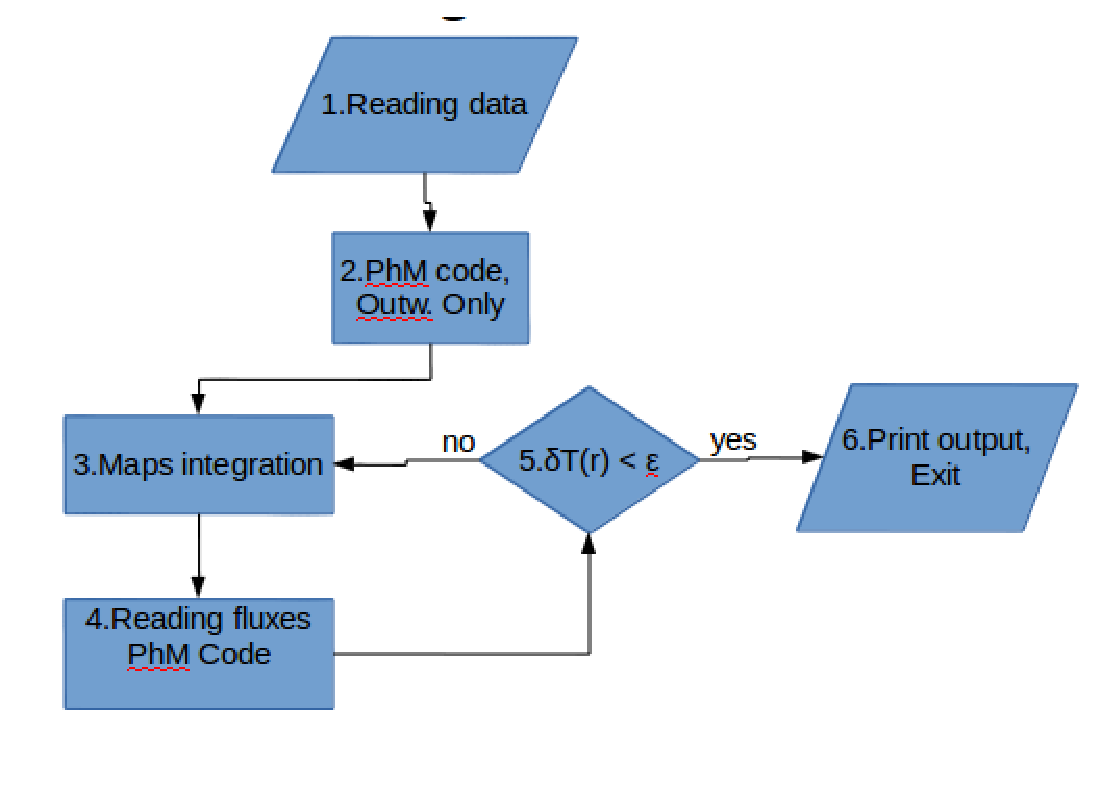
\epsfig{file = our_algo.eps,width = .85\linewidth}
\caption{Our approach algorithm}\label{our_approach}
\end{minipage}
\hfill
\end{figure}

\indent1 - Reading data, such as required precision, maximum iterations, etc.\\
\indent2 - Running PhM code in Outward Only mode, generating and saving emissivity and opacity maps.\\
\indent3 - Running integration procedure using previously generated maps.\\
\indent4 - Running PhM code, using fluxes, obtained after step 3. Generating and saving new emissivity and opacity maps.\\
\indent5 - Check difference between electron temperatures obtained from current iteration and the previous one. Once difference is greater than is required by precision, pointed in 1, then returning to step 3.\\
\indent6 - Printing fluxes and ionization structure, obtained from PhM on last iteration.\\


\section{DiffRay3D. General algorithm and limitations}

The current version of DiffRay3D provides tools for integrating radiation fluxes using 2D maps over a 3D volume (support for 3D maps will be implemented in future versions). The nebula is divided into 80 sectors (20 per quarter, assuming cylindrical symmetry, and physical conditions in each quarter are the same). Each sector is divided into slabs. The shell structure is defined from input emissivity/opacity maps.

General code algorithm is displayed below:

\begin{figure}
    \begin{minipage}[t]{.45\linewidth}
        \centering
        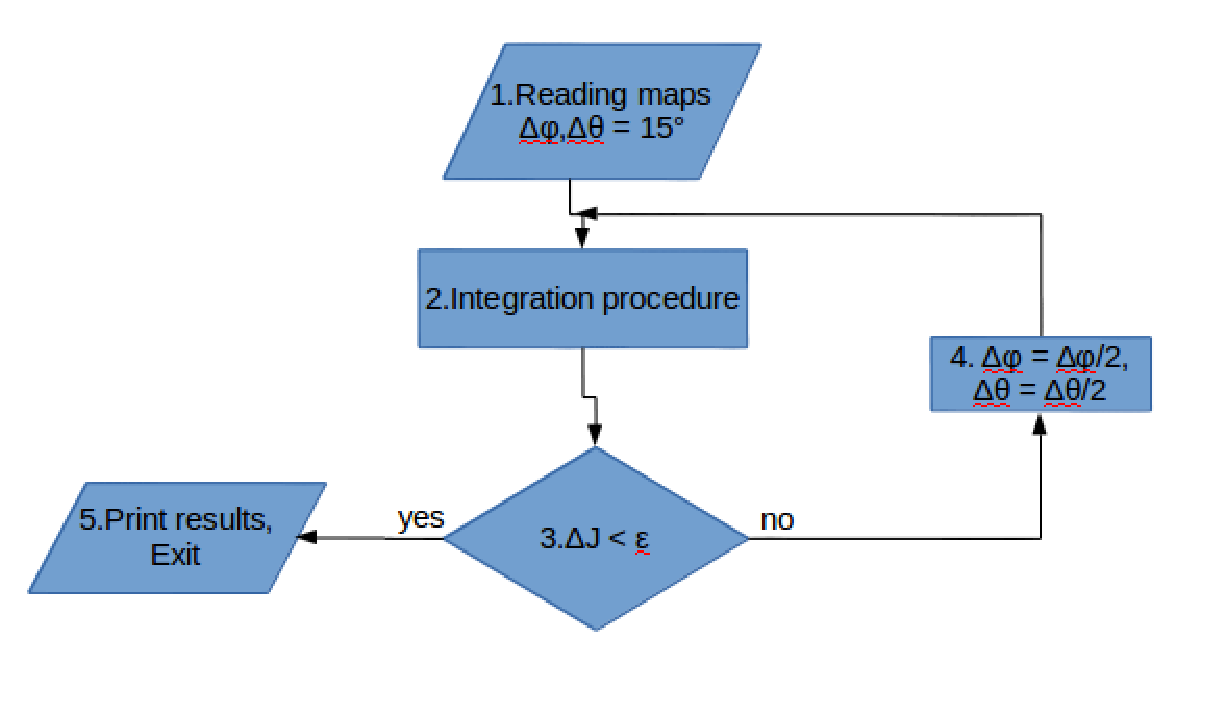
\epsfig{file = diffray_algo.eps,width = .85\linewidth}
        \caption{DiffRay algorithm}\label{diffray_algo}
    \end{minipage}
\end{figure}

For the implementation of the diffuse radiation fluxes integration procedure, the DiffRay code was developed. The code's algorithm is shown in figure \ref{diffray_algo}.\
\indent1 - Setting up initial integration steps for angles, reading emissivity and opacity maps that should be integrated.\
\indent2 - Integration of diffuse radiation fluxes for each elementary volume of the nebula environment.\
\indent3 - Comparing the difference between fluxes obtained on the current iteration and the previous one. If it fits the required precision, proceed to step 5. Otherwise, decrease the integration step (4), and return to step 2.\
\indent5 - Print fluxes in a format that can be read by the PhM code. Exit.\

\section{How to launch the code}

To run the code, you need a working compiled code version and valid object data with a commands file provided.

\subsection{Code compilation}

Download the code archive.\
Unzip files in any folder you wish. DiffRay3D can be started in any folder, the only requirement is that the code should have sufficient permissions to create/delete folders and files.\
Once unzipped, go to the "source/v*../" folder and run MakeFile.all. This will create the DiffRay3D.exe executable in the installation root folder.\
\section{Input data format}
To function correctly, the code must have information about the object's geometry, emissivity, and opacity maps, and so on. This information is read from the data folder. In general, the filename looks like:

Emis\_Lines\_SectorNo{\bf Sector number}\_Age{\bf Object age}Myr.dat

For example, Emis_Lines_SectorNo7_Age10.00Myr.dat

Here, the Sector number is the number of sectors represented by the file. The Age can be used as any identifier for the model data set. (For example, once you have maps for several models, you can enumerate them and use this enumeration in the age field.

A complete list of supported data files and their format can be found in the following subsections.

\subsection{Continuum Mesh}
{\bf Continuum{SectorNo}\_Last\_Age{ObjectAge}.dat} - a file with the continuum energy mesh structure. Each row should contain, in the first column, continuum cell energy in Rydbergs. The file is required. The structure of the file is as follows:
\begin{table}[H]
    \begin{tabular}{ll}
        cell 1 energy & \ldots \
        cell 2 energy & \ldots \
        cell 3 energy & \ldots \
        cell 4 energy & \ldots \
        \ldots & \ldots \
    \end{tabular}
\end{table}
Continuum cell energy should be represented in Rydberg units. The file can contain an arbitrary amount of columns, but only the first one is used, while the rest will be ignored. If you want to change the reading behavior, see the {\it CContinuum::readMesh} method in the "continuum.cpp" file.
\subsection{Continuum emissivities map}
{\bf Emis\_Cont\_SectorNo\{SectorNo\}\_Age{ObjectAge}.dat} - file with continuum emissivity data. Each row
corresponds to sector slab. First row has only one value - inner radius. Next rows contain slab outer radius in first column, 
and net volume emissivity values for each energy cell in corresponding slab in following columns. File is required. Note, that amount of columns in this file should
be equal to amount of rows in {\bf Continuum1\_Last\_Age{ObjectAge}.dat} + 1 column for radius.
The structure is following:
\begin{table}[H]
    \begin{tabular}{lll}
        inner radius & & \\
        Radius 1 & emissivity & \ldots \\
        Radius 2 & emissivity & \ldots \\
        Radius 3 & emissivity & \ldots \\
        \ldots & \ldots & \ldots \\
    \end{tabular}
\end{table}
Slab radius should be specified in centimeters. Emissivities are in $erg \cdot cm^-3 \cdot sec^-1$).
If you want to change reading behavour, see {\it CContinuum::readEmissivity} method in "continuum.cpp" file.

\subsection{Continuum opacities map}
{\bf Opac\_Cont\_SectorNo{SectorNo}\_Age{ObjectAge}.dat} - a file with opacity data for each continuum cell. Each row corresponds to a sector slab. The first row has only one value - the inner radius. Subsequent rows contain the slab's outer radius in the first column, and opacity values for each energy cell in the following columns. This file is used both for calculating continuum and line optical depths. The file is required. The structure is as follows:
\begin{table}[H]
    \begin{tabular}{lll}
        inner radius & & \
        Radius 1 & opacity & \ldots \
        Radius 2 & opacity & \ldots \
        Radius 3 & opacity & \ldots \
        \ldots & \ldots & \ldots \
    \end{tabular}
\end{table}
Slab radius should be specified in centimeters. Opacities are expressed in $cm^{-1}$.
If you want to change reading behavior, see the {\it CContinuum::readOpacity} method in the "continuum.cpp" file.

\subsection{Lines Emissivity}
{\bf Emis\_Lines\_SectorNo{SectorNo}\_Age{ObjectAge}.dat} - a file with lines emissivity data. Each row corresponds to a sector slab. The first two rows have headings, according to the standard Cloudy "punch line emissivity" command, \cite{Cloudy}. Subsequent rows contain the slab's outer radius in the first column, and emissivity values for each emission line in the following columns. The file is required. The structure is as follows:
\begin{table}[H]
    \begin{tabular}{llll}
        heading & & & \
        heading & line name & line name & \ldots\
        Radius 1 & emissivity & emissivity & \ldots \
        Radius 2 & emissivity & emissivity & \ldots \
        Radius 3 & emissivity & emissivity & \ldots \
        \ldots & \ldots & \ldots & \ldots \
    \end{tabular}
\end{table}
Slab radius should be specified in centimeters. Emissivities are expressed in $erg \cdot cm^{-3} \cdot sec^{-1}$.
If you want to change reading behavior, see the {\it CLines::readLines} method in the "lines.cpp" file.

    {\bf Important Note:} You can specify only lines defined in the known lines database. To check if a line exists and is supported, you can search the {\it data/database/line_ch.data} for the line label or in {\it data/database/line_en.data}. If you cannot find the desired line, you can add it by editing these files. It's highly recommended, however, to add any new lines at the end of the files. Also, if you edit these files, don't forget to copy them before you update DiffRay. Otherwise, the data you changed will be overwritten.

\subsection{Chemical Abundance}
{\bf Abund{SectorNo}\_Age{ObjectAge}.dat} - a file with elemental abundances data. Each row corresponds to a sector slab. The first row should have valid column headings with element names, provided as the first four symbols of the full name. (#Depth H HELI LITH BERY\ldots, Garry Ferland's Cloudy output format, see \cite{Cloudy}). Subsequent rows contain the slab's outer radius in the first column, and elemental abundances for each element in the following columns. This file is not required. The structure is as follows:
\begin{table}[H]
    \begin{tabular}{llll}
        Heading & Element 1 label & Element 2 label & \ldots\
        Radius 1 & Abundance Value & Abundance Value & \ldots \
        Radius 2 & Abundance Value & Abundance Value & \ldots \
        Radius 3 & Abundance Value & Abundance Value & \ldots \
        \ldots & \ldots & \ldots & \ldots \
    \end{tabular}
\end{table}
Slab radius should be specified in centimeters. Abundances are represented as $log_{10}(Element Particle Count / Total Particle Count)$. If you want to change reading behavior, see the {\it Abund::getElementList} method in the "abund.cpp" file.

\subsection{Physical Conditions Overview File}
\label{dataOverview}
{\bf Overview\{SectorNo\}\_Age{ObjectAge}.dat} - file with additional data about physical conditions. Each row
corresponds to sector slab. The first row is a heading.
(#Depth Te Htot hden eden \ldots, Garry Ferland's Cloudy output of the {\it punch overview}
format, see \cite{Cloudy}). Subsequent rows contain the slab's outer radius in the first column,
and corresponding values, like electron temperature, electron density, and so on. The structure is as follows:
\begin{table}[H]
    \begin{tabular}{llllll}
        Heading & & & & & \
        Radius 1 & Electron Temperature & Heating Rate & Density & Electron Density & \ldots \
        Radius 2 & Electron Temperature & Heating Rate & Density & Electron Density & \ldots \
        Radius 3 & Electron Temperature & Heating Rate & Density & Electron Density & \ldots \
        \ldots & \ldots & \ldots & \ldots & \ldots & \ldots \
    \end{tabular}
\end{table}
Slab radius should be specified in centimeters. Physical values are mostly represented on a logarithmic scale. If you want to change reading behavior, column order, and so on, see the {\it Physics::readPhysics} method in the "physics.cpp" file.

\section{Commands file}

Once you have compiled the code and prepared the data files, you should write some instructions for how and what the code should calculate. These instructions are contained in the commands.ini file in the installation root directory.

An example is distributed with the code source. \

\subsection{IO settings}
{\it print directory "path to your output folder, relative to the installation root directory"} - set the path to the folder where output files will be located\
    {\it input directory "path to input data files folder, relative to the installation root directory"} - set the path to the folder with input data\

    {\bf Example:}\
print directory result/ngc/ism0/140\
input directory data/ngc1569nograin\
Please note that paths should be provided without quotes!\

\subsection{Geometry and distance}
Commands that control the object's position in space.
    {\bf Distance}\
    {\it distance log10_dist units}.\

    {\bf Example:}\
distance 19.87 km \
(The distance to the object is adopted to be $10^{19.87}$ kilometers.
Supported units are meters, kilometers, centimeters.

    {\bf Object}\
    {\it object phi x}, x - object's azimuthal rotation angle relating to the observer's sight ray in radians;\
    {\it object theta x}, x - object's vertical rotation angle relating to the observer's sight ray in radians;\
    {\it object age x}, x - object age, or another model's bundle identifier; Currently, it doesn't have any impact on calculations.\

    {\bf Example:}\
object phi 0.76\
object theta 0.21\
object age 50\

\subsection{Calculation and integration options}
{\bf Integration}\
    {\it integration maxiterations x}, x - maximum code iterations. This option is useful to prevent the code from falling into an endless loop when trying to converge.\
    {\it integration precision x}, x - acceptable convergence between iterations, 0.01 - 1%. \
    {\it integration mode outw} - switches code to Outward Only mode, is good for tests.\
    {\it integration predictive on} - turns on an additional iteration that runs before the main process of splitting the object into spatial angles and solving
radiative transfer for those. This step tries to predict how much fluxes are changed along different sightlines within some angular sector
to determine the desired initial angular integration step. It is recommended to turn on only in the case of an object with complex geometry and/or
significant spatial inhomogeneities.

{\bf Example:}\\
integration precision 0.005\\
integration maxiterations 12\\
integration predictive off\\

{\bf Calculation}\
calculation {scope} on/off - controls what kind of calculations DiffRay should perform. \
    {\it calculation opacity on/off} - turn on/off opacity calculation (turning this off assumes that the environment is very optically thin for all
quantum) \
    {\it calculation continuum on/off} - turn on/off radiative transfer for the continuum. Turning off will make DiffRay calculate only line fluxes. \
    {\it calculation abundance on/off} - turn on/off calculation of weighted elemental abundances within the volume cut by the aperture/along the observer sightline. Once you turn this on,
abundance data files are required (See \ref{dataAbund} for details). \
    {\it calculation overview on/off} - turn on/off calculation of average electron temperature and density within the volume cut by the aperture/along the observer sightline. Once you turn this on,
overview data files are required (See \ref{dataOverview} for details). \

\subsection{Isophotes}
isophote {line | ratio} {line label} - prints a map of fluxes for a selected line within a square cut by the aperture. \
This can be useful to visualize the spatial distribution of modeling volume brightness in specific emission lines. \
    {\it isophote line 'line label'} - prints a map of absolute fluxes for a selected line. \
    {\it isophote ratio 'line label'} - prints a map of relative fluxes for a selected line ($F(selected line)/F(H_{\beta})$). \

\subsection{Aperture}

{\it aperture phi theta w h} - Adds an aperture to the list of apertures to be calculated.
Here phi - azimuthal aperture position, theta - vertical position relative to the ray
from the observer to the center of the object. w, h - aperture width and height. All values
should be provided in radians.\

    {\bf Example:}\
aperture add 0 0 0.000014537 0.000014537\
aperture add 0.000464 0.0000139 0.000014537 0.000014537\
aperture add -0.000271 -0.0000102 0.000014537 0.000014537\
In this example, the code will run calculations for 3 apertures, and put results in the
app{N} folder. N is the aperture number here. Aperture folders are created automatically
in the directory specified with the output command.

\section{Output}
Output files will be stored in the output directory specified in the corresponding commands file command.

\subsection{Emission Lines Results}
{\bf linesarr.dat} - a file containing fluxes for each line specified in the line emissivities input file (see \ref{dataLines}).
Each row contains four columns: line label, Flux at observer ($\mathrm{erg} \cdot \mathrm{cm}^{-2} \cdot \mathrm{s}^{-1}$), Luminosity ($\log_{10}(\mathrm{erg} \cdot \mathrm{s}^{-1})$),
and relative flux ($F(\text{line})/F(H_{\beta})$).\\
{\bf llum.dat} - an alternative representation of line luminosities. The file contains only two rows: a header, and luminosities for each line specified in the line emissivities input file (see \ref{dataLines}).
Luminosity is printed as ($\log_{10}(\mathrm{erg} \cdot \mathrm{s}^{-1})$). \\
{\bf lifr.dat} - an alternative representation of line fluxes. The file contains only two rows: a header, and fluxes for each line specified in the line emissivities input file (see \ref{dataLines}).
Fluxes are printed as ($\mathrm{erg} \cdot \mathrm{cm}^{-2} \cdot \mathrm{s}^{-1}$).

\subsection{Continuum Output}
{\bf contarr.dat} - contains continuum fluxes at different photon energies. It contains three columns:
1 - Photon energy, 2 - amount of quanta of attenuated incident continuum ($\mathrm{cm}^{-2} \cdot \mathrm{s}^{-1}$), 3 - amount of quanta of diffuse continuum ($\mathrm{cm}^{-2} \cdot \mathrm{s}^{-1}$).\\

More output files with additional formats are planned for the future.

\subsection{Chemical Abundances}
{\bf abmass.txt} - contains the abundances of elements within a volume cut by an aperture within the object, weighted by mass.
It has two rows: a heading and a list of weighted abundances ($12 - \log_{10}(n(\text{element})/n(H))$). \\
{\bf abemso.txt} - contains the abundances of elements within a volume cut by an aperture within the object, weighted by oxygen
lines emissivity ($e(O3  5007\text{\AA}) + e(O3  4363\text{\AA}) + e(O3  4959\text{\AA}) + e(O2  3726\text{\AA}) + e(O2  3729\text{\AA})$).
It has two rows: a heading and a list of weighted abundances ($12 - \log_{10}(n(\text{element})/n(H))$).

\subsection{Isophotes}

{\bf isophote\_\{index\}.dat} - file containing 2D data for drawing flux maps.
The 1st and 2nd columns represent spatial angles, and the 3rd column lists the fluxes calculated from the direction determined by these spatial angles. \\

When 'isophote' commands are present, gnuplot scripts for visualization are generated and located in the "plots"
folder within your output directory.


\begin{thebibliography}{3}
{\small
\bibitem{DIAGN} Golovaty V.\,V., Dmiterko V.\,I., Mal'kov Yu.\,F., \& Rokach O.\,V. 1993, Astronomical Report, Vol. 37, Issue 4, pp. 346-354
\bibitem{JPS2016} O. S. Buhajenko, B. Ya. Melekh 2016, `METHOD FOR DETAILED CALCULATION OF THE DIFFUSE IONIZING RADIATION IN NEBULAR ENVIRONMENTS`, Ivan Franko National University of Lviv, 4901 (13 p.) 
\bibitem{Cloudy} Ferland G.J. 1999, `Hazy, a Brief Introduction to Cloudy 94`, University of Kentucky, Physics Department Internal Report; \texttt{http://www.nublado.org}
}
\end{thebibliography}
\end{document}
